\section{Work Efficiency Metric} \label{sec:metric}

In this section we define work efficiency, a metric for comparing different optimized versions of a program when executing with different
inputs. We define it as the ratio between the amount of \textit{work}, $\Delta W$, performed during a period of time, $\Delta t$.

\[
   P = \nicefrac{\Delta W}{\Delta t}
\]

The main challenge is to precisely define what represents \textit{work}.
We define the work done by a program on an input to be the time taken by the unoptimized program to process that input.
We estimate the runtime of each instruction type via a linear regression and then define the work done by a program as the sum of the

We adopt a work metric that takes into account the
computational cost within each basic block.
The computational cost of a basic block is given by weighting the instructions
that it contains.

To this end, we model the computational work $\Delta W$ as a linear equation based on block frequency information and a cost model of the instruction set.
Formally,
\[
\Delta W = \varepsilon + \sum_{B} w(B)f(B)
\]
where $f(B)$ represents the frequency of basic block $B$ and $w(B)$ represents the computational work of executing $B$.
We define the work of a basic block $B$ as the sum of the cost of its instructions, i.e.,
\[
w(B) = \sum_{i} w_i N_B(i)
\]
where $w_i$ is the cost of instruction $i$ and $N_B(i)$ is the number of occurrences of instruction $i$ in basic block $B$.

In this simplified model, we consider that $w_i$ is constant across all programs and executions, varying only between target architectures.
On the other hand, $N_B(i)$ is a program-dependent static value which is known at compile-time and $f(B)$ is a dynamic value known only at run-time,
since $f(B)$ is both program and execution dependent as the execution frequency of a basic block can change when executing with different inputs.

\subsection{Estimating a Cost Model of the Instructions}

Similarly to previous work~\citep{giusto01,powell09,brandolese11}, we derive the cost model of the instruction set by modeling the problem
as a multi-variable linear regression. The \textit{regression coefficients} are the costs of the instructions and the \textit{regressors}
are computed as $\sum_B N_B(i)f(B)$ for each instruction.
\begin{equation}\label{eq:linear-work-expression}
\Delta W = \varepsilon + \sum_{i} \left(w_i \sum_{B} N_B(i)f(B)\right)
\end{equation}

We use a set of training programs to construct the regression model. Our training program set is given in
Table~\ref{tab:kdatasets:training}. To determine the model coefficients, we profile each training benchmark with 1000 input datasets
provided by the benchmark suite, and we measure the wall-clock time. It is to note that we turn off all compiler optimisations during this
training stage, to ensure that the amount of work we measured only depends on the program input but not compiler optimization. This aspect
is crucial for the work-based performance metric to allow a consistent comparison between the various optimization sequences when executing
with distinct inputs.


%it allows to use the estimated cost model for computing a work metric which is independent of optimizations, as we explained in Section~\ref{}.

Our cost model has a total of 52 LLVM instructions\footnote{We do not model all LLVM instructions because some instructions are more common in optimized programs, such as the vector instructions.}.
Every program, in the set of training benchmarks, was compiled twice: once including the necessary instrumentation for the block frequency profiling, which is required for deriving the linear expression defined in Equation~\ref{eq:linear-work-expression};
and a standard compilation without any optimization or instrumentation.
For each input in the training dataset, the benchmarks were executed once with the instrumented version for collecting the block frequency profiling, and multiple times with the standard compilation just for measuring the wall-clock execution time, until the confidence interval was no larger than 1\% for a 99\% confidence.
After collecting these measurements, this data can be used to estimate the unknown parameters in the linear model.
Because we fit the linear model based on the wall-clock execution time, the derived cost model can be interpreted as an estimate of the execution time when the program is compiled without optimizations.

\begin{figure}[t]
    \centering
    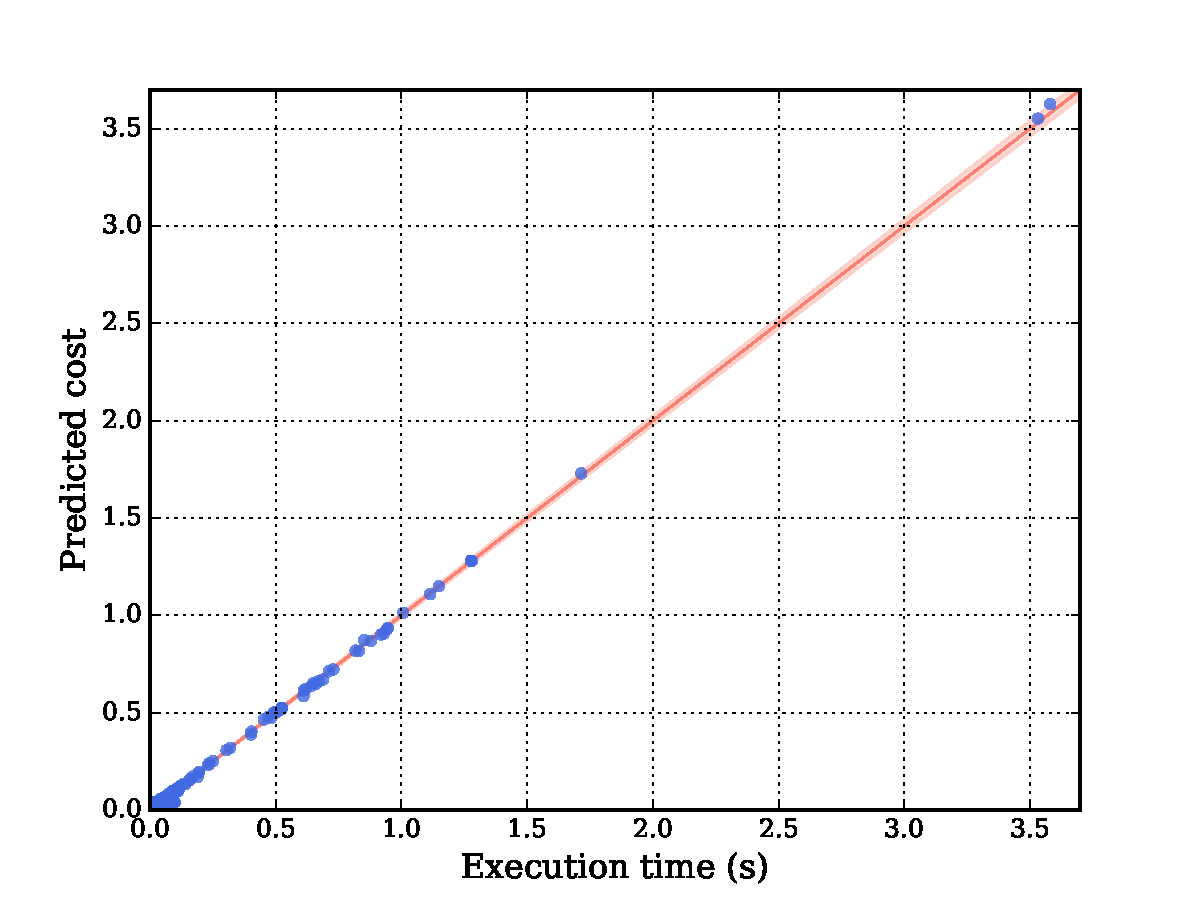
\includegraphics[width=0.6\linewidth]{figs/cost-model.pdf}
    \caption{Linear model fitted from empirical data. The mean absolute error (MAE) for the fitted curve is seven milliseconds.}
    \red{zw: bigger font size.}
    \label{fig:cost-model}
\end{figure}

Figure~\ref{fig:cost-model} compare the work metric with the corresponding execution time for some instances of the test benchmarks.
Notice how the fitted model has a higher relative error for the instances with very short execution time, namely those that run for less than one tenth of a second.
The mean absolute error (MAE) for the fitted curve is seven milliseconds.

\begin{figure}[t]
    \centering
    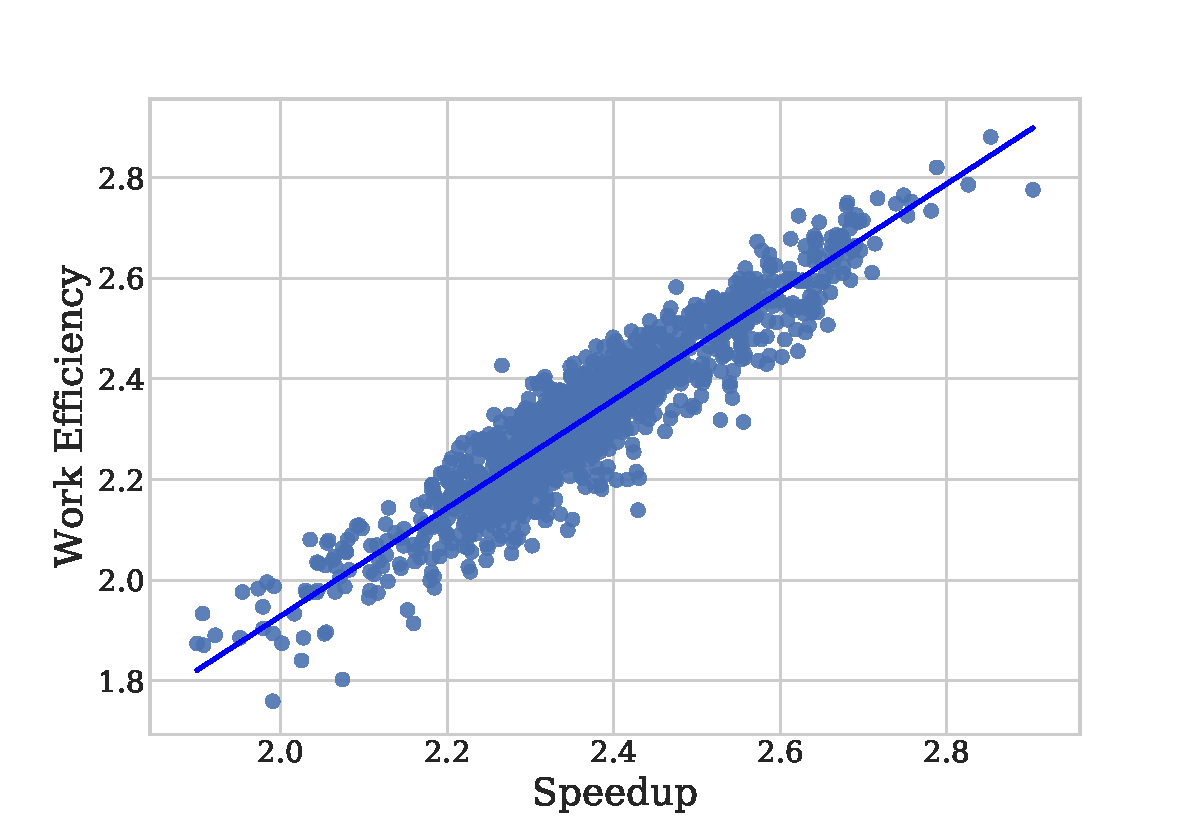
\includegraphics[width=0.5\textwidth]{figs/motivation-work-efficiency.pdf}
    \caption{Relationship between work efficiency vs speedup for 500 different binaries of \texttt{susan\_c}.
            Each point represents averages over a subset of all inputs.}
    \label{fig:motivation-work-efficiency}
\end{figure}

\FIXME{Rodrigo: I think we could show how the work efficiency metric performs compared with speedup, the same way we showed the other metrics does not work well.}

\subsection{Comparison with Instructions Per Cycle} \label{sec:ipc-vs-work-metric}

\FIXME{Rodrigo: Perhaps we could remove this section, since we have already discussed the IPC in the Motivation.}

The IPC metric has been widely used for studying performance benefits of hardware optimizations.
Although previous work has suggested the use of IPC for guiding {\itercomp}, in this section we argue in favour of the WP metric over IPC.

The IPC metric differs from the proposed WP metric in a key aspect:
the IPC metric is computed solely based on the final optimized program.
When executing different optimized versions of a program with the same input, both the number of instructions and the number of clock cycles can change.
For this reason, higher IPC does not necessarily translate to shorter execution time (or even fewer clock cycles).

% We can illustrate this fact with a very small example as shown in Table~\ref{tab:ipc-example}.
% This example shows two versions of a program, namely P1 and P2, and their respective measurements related to IPC.
% Although version P1 has twice the IPC of P2, P1 is one cycle slower than P2.
% As this example illustrates, the IPC metric can be misleading when compared different versions of the same program.
% This problem is only intensified when both the optimization sequence and the input changes.
% In Chapter~\ref{chap:eval} we show empirical evidence for this argument.
%
% \begin{table}[h]
% \centering
% \begin{tabular}{|c|c|c|c|}
% \hline
%                        & P1 & P2  \\
% \hline
% Number of Instructions & 5  & 2   \\
% Number of Cycles       & 5  & 4   \\
% IPC                    & 1  & 0.5 \\
% \hline
% \end{tabular}
% \caption{Example that illustrates that a higher IPC does not necessarily translate to shorter execution time.}
% \label{tab:ipc-example}
% \end{table}

On the other hand, WP computes the amount of work based on the unoptimized version of the program, which means that it always measures the same amount of work for the same input, regardless of the optimizations applied on the program.
This is a key aspect that enables the use of the WP metric for guiding {\itercomp}, because a higher WP, which represents work per unit time, naturally translate to shorter execution time.
Moreover, previous work has also presented other arguments against the use of IPC in similar use-case scenarios. %, as discussed in Chapter~\ref{chap:related}.
